% Proposed solution

\chapter{Implementation} \label{ch:impl}
This chapter provides a detailed explanation of how the project was implemented from the environment set-ups to the automation and execution of that automation.
It outlines the practises, techniques, and steps taken to bring the project to completion.
Metropolia University of Applied Sciences provided a LORIX One gateway, a micro\gls{sd} card with ChirpStack Gateway \gls{os} full image installed to it, a spare micro\gls{sd} card and two complete \gls{lora} end devices, that are used by the students in the courses the project is implemented for. Two extra \gls{lora} radio modules were also provided as the board provides a possibility to have two modules connected into it.

The source code for the implementation can be found in Appendix~\ref{appx:sourcecode}.
Sensitive information in variables, like password, is replaced with dummy versions.

\section{Setting up LORIX One}
The LORIX One gateway is used to establish the connection between the ChirpStack Network Server and the \gls{lora} devices.
The gateway came together with a micro\gls{sd} card where the ChirpStack Gateway \gls{os} image was already installed.
The LORIX One has a slot for the micro\gls{sd} card inside where it was put.
After that the LORIX One was connected to a router to get Ethernet access and to an outlet to get power.
When the gateway is powered it starts the boot immediately meaning in this case the ChirpStack Gateway \gls{os} image.

\clearpage

\section{Setting up ChirpStack}
When the connection is stable in the LORIX One gateway and its status led blinks on a heartbeat mode the \gls{os} installation can be started.
The \gls{os} is booted each time it is connected to a power supply and the user needs to login using \gls{ssh} to access the ChirpStack \gls{os}\cite{chirpstack:gettingStarted}.
The command requires the username and the \gls{ip} address for the server as seen in Figure~\ref{fig:ChirpStack_gateway_os}.
The Username was provided by the school and the \gls{ip} address was verified through the connected devices of the router.

\begin{figure}[ht]
  \centering
  {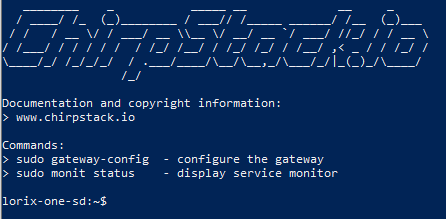
\includegraphics[width=\textwidth]{illustration/chirpstack_io_main_screen.PNG}}
  \caption{Interface layout of ChirpStack Gateway OS full, when the user has logged in}
  \label{fig:ChirpStack_gateway_os}
\end{figure}

As mentioned earlier the micro\gls{sd} card was provided with the ChirpStack \gls{os} and also with the needed credentials to log in.
The data the card contained the latest settings that Metropolia University of Applied Sciences uses and new configurations were not needed.
The command prompt was closed with an exit command.

\section{Creating Excel file for end devices}
The Excel file format was selected for storing the information about the application name and its details and all the devices that it should have in it.
The decision to utilize an Excel file was selected due to a accessibility of a pre-existing library called RPA.Excel.Files in Robot Framework.

\clearpage

The Excel file, \path{Applications.xlsx}, layout was designed so that each sheet the file includes would be named after the application name that the sheet contains.
When a sheet is opened it has three headers focusing on the application in the first row.
Those headers are called Application name, Application description and Service profile.
On the second row under each header of the columns the information is stored accordingly so that the data can be fetched by using the headers.

Row four contains headers for adding a \gls{lora} device to the application.
Those headers are called Device name, Device description, Device \gls{eui}, Device-profile and Application key.
Under those headers the user adds the device information correspondingly.

The Device \gls{eui} consists of 16 digits and/ or characters that can be given using three different forms, all written together, or with whitespaces, or colons as separators.
The parsing of colons and whitespaces is handled by ChirpStack.
The restrictions for the \gls{eui} code are that it can not include special characters in any form, as they are ignored by ChirpStack.
When the \gls{eui} is given to the corresponding field and a lack of correct amount of accepted digits and/ or characters, it results to an error when the device is tried to be added.

The Excel file filling is fully manual and left to the educator to fill in, but for this project three mock up sheets were created to test that the functionality works correctly.

\section{Creating automation}
This section will give an overview of how the automation was created for the project.
The automation was done using Robot Framework in the Visual Studio Code source code editor as it provides the possibility to implement Robot Framework and Robocorp extensions that were used.

The first step to start the automation was to build up the project structure for the ease of maintenance.
The project directory contains two main folders called automation and resources alongside with the \path{.gitignore} file and the \path{requirements.txt} file.
The automation folder contains the two robot files used for the automation, \path{__init__.robot} and \path{automation.robot}.
The resources folder is used in this project to store the \path{variables.py} file which is used in the project.
All the required packages and libraries are included in the \path{requirements.txt} file.

\subsection{variables.py}
The \path{Variables.py} is a python file where all the variables are stored to easily modify them if needed from one place.
The \path{variables.py} file includes a list of variables that are used in the suite setup and teardown, but also in the process automation.

All the variable names were created using uppercase characters and snake case in the naming to provide a better readability and recognition of the origin of the variables.
The variables used and crea\path{automation.robot} file were created with low case characters witted in the h the same snake case style.

A mockup version of the file is provided in Appendix~\ref{appx:sourcecode} to see what kind of formats were used.

\subsection{Suite Setup and Suite Teardown}

In this project Suite setup was selected to be utilized to eliminate unnecessary repetition of steps to be taken and to verify the pre-steps are functioning correctly before the tasks are run.
Suite setup was utilized in a suite initialization file called \path{__init__.robot} file which is run once and before files of the automation folder are executed.

The Suite Setup setting that was implemented is called Login to ChirpStack.
The task opens the browser with the browser type that was specified in the \path{variables.py} file.
For running the automation with a window where the user can see the progress while it runs, the headless argument was set to false.
When the browser is opened the next keyword takes the \gls{ip} address of the ChirpStack server for the login page that was initialized in the \path{variables.py} file.
The code then proceeds to fill the text fields for username and password also with values that were initialized in the \path{variables.py} file.
When the login credentials have been filled the task clicks the Login button.
Web elements, like the Login button, have been identified with selectors, mostly using the xpaths of those elements.
Some required a text identifier beside them to recognize them when an xpath is the same with another element.
The task then uses keywords to save the \gls{url} of the updated page to a variable and then compares it to the expected \gls{url}.
Lastly, the amount of items on a page of the applications list is set to be 100.

When the \path{automation.robot} file is executed the logs show if the setup passed alongside with the tasks.
If the suite setup fails the tasks will also be set to fail status\cite{robotFrameworkUserGuide:suiteSetupAndTeardown}.

The Suite Teardown setting is called Log out from ChirpStack.
The teardown navigates to the Logout button by pressing the username on the top right corner of the web interface and clicks the  Logout button.
The browser is then closed.

Suite teardown is executed after all test cases and child suites of a test suite are run.
It is always run no matter what the execution results of the test cases are or if the suite setup has failed.
If the teardown fails, all the tests of the test suite are set to fail status\cite{robotFrameworkUserGuide:suiteSetupAndTeardown}.

\subsection{Process automation}
The \path{automation.robot} file consists of tasks that were used for creating the application, adding and deleting devices and to delete a selected application.

The file has one task called main which executes a keyword named \textit{Take User Input}.
\textit{Take User Input} asks the user which of the named four tasks, seen in Figure~\ref{fig:user_input_commands}, is to be executed and after the selection the corresponding actions are made.
For utilizing these tasks four Robot Framework libraries were imported in the settings section: Browser, Dialogs, RPA.Excel.Files and Collections.

\clearpage

\begin{figure}[ht]
  \centering
  {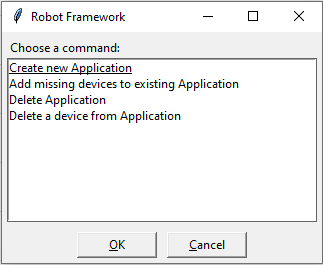
\includegraphics[width=10cm]{illustration/take_user_input_dialog.PNG}}
  \caption{Dialog pop-up window, where the user can select the task they want to be executed}
  \label{fig:user_input_commands}
\end{figure}

When \textit{Take User Input} is run, a list is acquired from the \textit{Get Application elements as lists} keyword.
The keyword goes through all the applications that are listed on the Applications layout of the ChirpStack Application server.
Each list item contains the ID, name, service-profile and description of the application.
The information of them is stored as elements in four separate lists by the header types.
Those four lists are then added to another list which is returned when the keyword is run.
The returned list is then used to access all the application name elements.
The elements are then used to access all the application names with a \textit{Get Application Names} keyword.

The \textit{Get Application Names} keyword takes a list of application name elements as an input and goes it through while saving each element in the corresponding application name in the Applications layout on ChirpStack.

After the application names are saved on a list a user input is asked to select what command is to be executed.
The commands are using the \textit{Get Selection From User} keyword of the Dialog library\cite{robotFramework:dialogsLibrary}, that shows a list of the named selection options in a pop-up window.
When that is selected the \textit{Take User Input} task proceeds to find the corresponding command name from an if--else statement and actions inside the statement are run after.
The following sections walk through all the commands and what their content consists of.


The Create Application command is the first one on the list of selections the user can take.
It saves all the existing worksheets from the \path{Applications.xlsx} file using the \textit{List worksheets on Excel} keyword of the RPA.Excel.Files library\cite{rpaFramework:excelFiles}.
After that \textit{Remove Already Existing Application Names from Sheet Options} is run with two list inputs, the list of Excel worksheets and another with the existing application names, which were obtained when the task begun to run.

\textit{Remove Already Existing Application Names from Sheet Options} goes through the application names from ChirpStack using a for-loop. The loop compares the current application name to the list of worksheet names from the Excel file and if a match is found, the application name is removed from the worksheet names.
This keyword is used to remove all the application names that already exist in the ChirpStack server from the list of options, from where the user can select the new application from.

The returned list from \textit{Remove Already Existing Application Names from Sheet options} is then inspected.
If the list size is zero, there are no new applications to add from the Excel file and a text input is added to the list and given as a selection to the user to exit the program.
If there are worksheet names left on the list instead, the program proceeds to provide another list of selections to user.
This pop-up window asks the user to select which application from the options the user wants to add and lets the user know of possibly removed options.
Figure~\ref{fig:new_application_select_application} provides screenshots of both dialog options mentioned above.
When the application name is selected the \textit{Create Application} keyword is run with the name as an input.

\clearpage

\begin{figure}[H]
  \centering
  \begin{tabular}{@{}c@{}}
    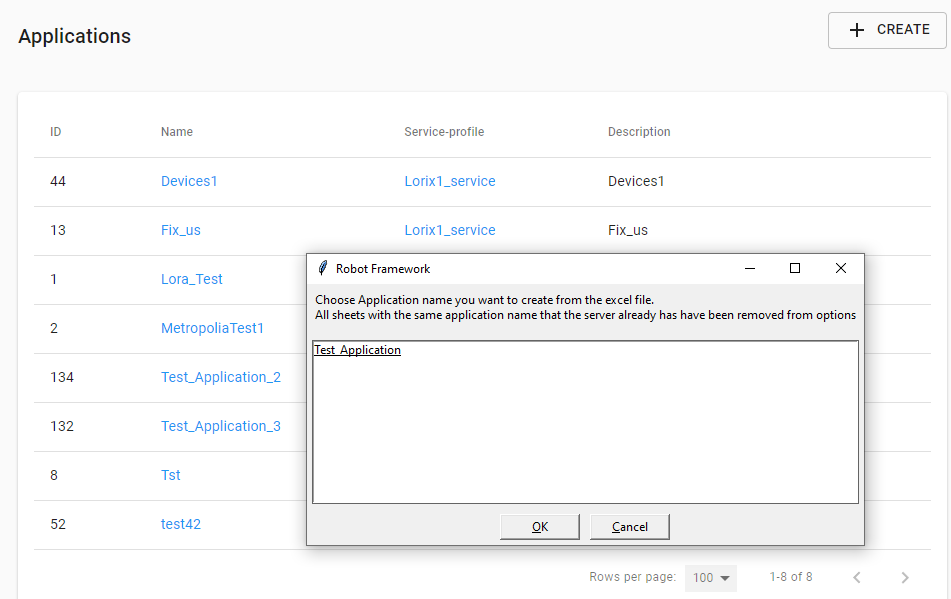
\includegraphics[width=\textwidth]{illustration/create_new_application_choose_application_dialog.PNG} \\[\abovecaptionskip]
    \small (A) Dialog pop-up window, where the user can select the application they want to create, \\ based on what applications from the Excel sheet are already added to the server
  \end{tabular}

  \vspace{\floatsep}

  \begin{tabular}{@{}c@{}}
    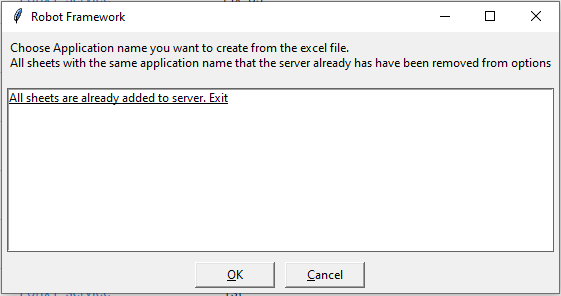
\includegraphics[width=12cm]{illustration/all_sheets_are_already_added.PNG} \\[\abovecaptionskip]
    \small (B) Dialog pop-up which is shown when all the applications from the Excel file are already added to \\ the ChirpStack server
  \end{tabular}

  \caption{Dialog pop-up is shown to the user when they select the Create Application command. Two variations of the content are available depending on what applications are already added from the Excel file.}\label{fig:new_application_select_application}
\end{figure}

\clearpage

\textit{Create Application} opens the worksheet of the \path{Applications.xlsx} file that has the given application name.
The name is verified to be there, as the list of selection was based on the worksheet names of this file.
First the Create button is clicked to access the create application layout.
The keyword then uses the keywords of the RPA.Excel.File library to save the worksheet as a table and to read the cell values from the second row of the worksheet, to access the application details which are added to the corresponding fields on the web interface.
When the new Application is created the layout changes to the list of all applications.
The keywords to access the application names are used to verify the newly created application is added and to access its name element.
The name element is then used with the \textit{Open Application} keyword to access the application and to add the devices from the worksheet.

The \textit{Add Devices} keyword is run from the opened layout of the  application.
It opens the Excel file from a worksheet with the same name as the application and saves the device information of all devices as a table.
The table is then gone through with a for-loop to use the \textit{Add One Device} keyword to save the devices one by one.
\textit{Add One Device} opens the device creation layout and fills in the required information to the web interface it has got from the Excel file.
If a device already exists, it means there is a device with the same name on the same application already, or a device with the same \gls{eui} is already added to the server.
If the problem lies with the two identical device names in the same application, the second one that is tried to be added is just ignored and the keyword returns.
If that is not the case, the keyword proceeds to use the \textit{Find a Device EUI from Application Names} keyword to find in which application it already exists on.
That application name is saved by the keyword and saved to the worksheet of the application from where the device was tried to be added.
This way the educator can easily see from the row of the device the device location on the server and remove it if needed.
If there was a problem adding the device \textit{Add One Device} returns to the application layout to proceed to add the rest of the application.
When all the devices are added the Create Application command is finished.

The second command in the Get Selection From User keyword of the \textit{Take User Input} task is called Add missing devices to existing Application.
This command lists all the applications that are already added to ChirpStack from the Excel file.
That list is then provided to the user using the same \textit{Get Selection From User} keyword from the Dialogs library \cite{robotFramework:dialogsLibrary} as mentioned earlier.
The selected application is then opened and the \textit{Add Devices} keyword is called.
\textit{Add Devices} is a suitable option for this command as well for its previously mentioned feature to ignore all the devices with an identical name on the selected application.

The third command in the \textit{Take User Input} is called Delete Application.
The command lists all the existing applications on the web interface for the user to select the one to delete, as seen in Figure~\ref{fig:delete_application}.

\begin{figure}[ht]
  \centering
  {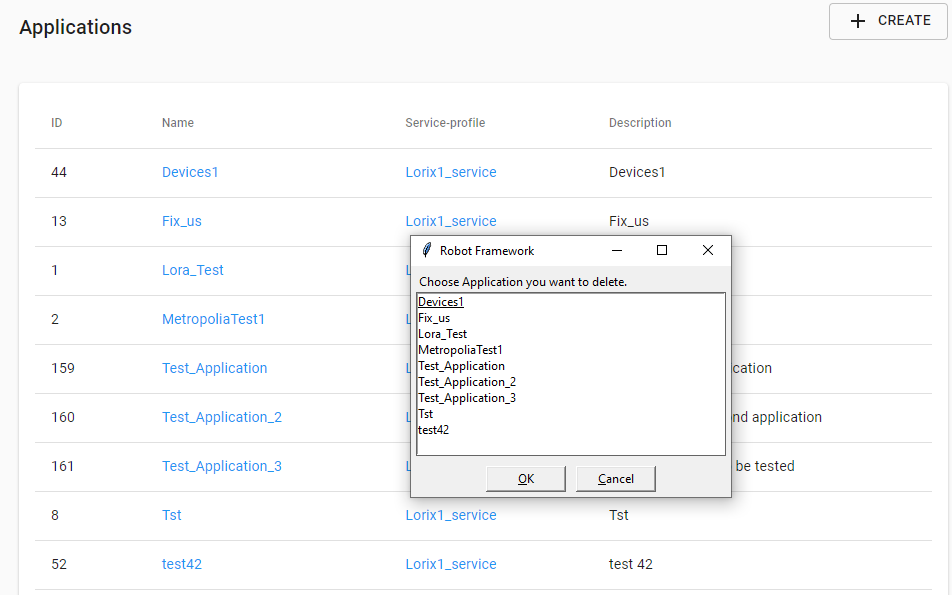
\includegraphics[width=\textwidth]{illustration/delete_app_choose_app_dialog_with_applications_on_back.PNG}}
  \caption{Dialog pop-up window, where the user can select the application they want to delete, based on what applications already exist on the server}
  \label{fig:delete_application}
\end{figure}

The last of the commands in \textit{Take User Input} is named Delete a device from Application.
It lists all the existing applications from the ChirpStack server for the user to make the selection, as seen in Figure~\ref{fig:delete_device_select_application}.

\clearpage

\begin{figure}[ht]
  \centering
  {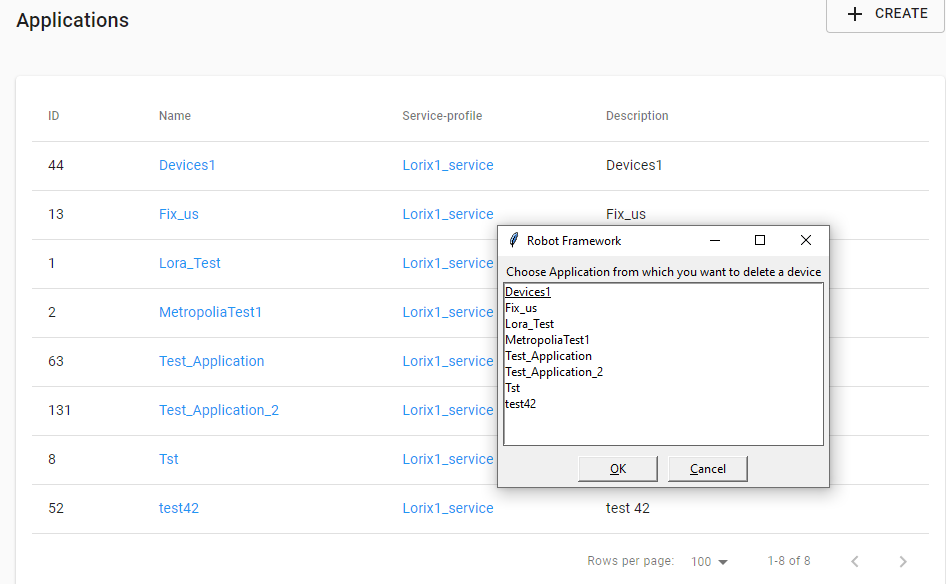
\includegraphics[width=\textwidth]{illustration/delete_device_choose_app_dialog_with_applications_on_back.PNG}}
  \caption{Dialog pop-up window, where the user can select the application they want to delete the device from, based on what applications already exist on the server}
  \label{fig:delete_device_select_application}
\end{figure}

After the application is selected, the command proceeds to list all the devices in a similar way, as seen in Figure~\ref{fig:delete_device_from_application_choose_device}.
If the application has no added devices, the command offers possibility to delete the application instead.

\begin{figure}
  \centering
  \begin{tabular}{@{}c@{}}
    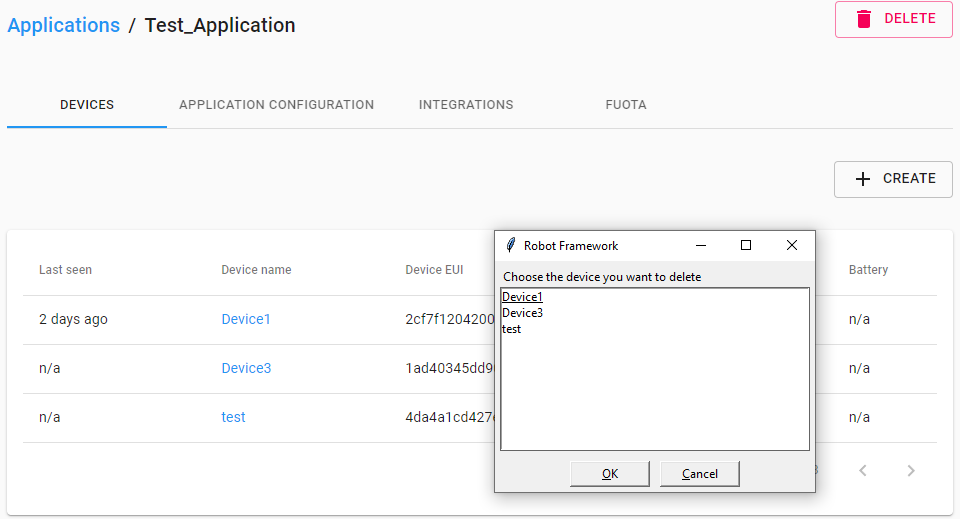
\includegraphics[width=\textwidth]{illustration/delete_device_from_app_choose_device_dialog_application_on_back.PNG} \\[\abovecaptionskip]
    \small (A) Dialog pop-up window, where the user can select the device they want to delete. \\ The list is based on what devices are added to the selected application on the server.
  \end{tabular}

  \vspace{\floatsep}

  \begin{tabular}{@{}c@{}}
    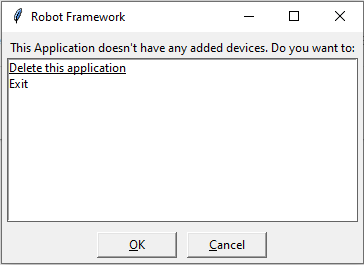
\includegraphics[width=10cm]{illustration/no_devices_to_delete.PNG} \\[\abovecaptionskip]
    \small (B) Dialog pop-up window, which is shown when there are no devices \\ to delete in the selected application.
  \end{tabular}

  \caption{Dialog pop-up window options, when the user selects the Delete a device from Application command. The window varies depending if there are any added devices on the chosen application.}\label{fig:delete_device_from_application_choose_device}
\end{figure}

\clearpage

\subsection{Testing}
When the implementation was done testing the functionality and comparing the efficiency could be done.
The functionality was tested by running the commands through with all the options used.
The \gls{lora} end device details were added to the Excel file and the devices were plugged to a power source to run the Python scripts to boot the devices.
Usually the students use one \gls{lora} module attached to a board, but to test more devices two modules were used in one board and two boards were provided for the testing purposes, so four devices in total were tested.
For this reason the Python script needed some modifications as it was implemented to boot one device only.
One of the updated scripts can be found from Appendix~\ref{appx:testing}.
The other one only has different application key defined to one of the devices, so one variable value is different.
After the devices were added to ChirpStack they could be manually accessed from the web interface.
From there the device details could be checked together with the data transmitting.
The devices were added to two of the three applications that were in the \path{Application.xlsx} file.
One of the devices had been defined with a different application key in both the Python script and the Excel file.
All the devices were successfully connected to ChirpStack and were transmitting data simultaneously as expected.

Efficiency was tested by running the Create Application command in different ways and by measuring the execution time.
This was done by creating three applications in each method, and the applications had a different amount of devices to see the differences in a longer run.
The first application had five devices, second 20, and third 45.
The first test run was done manually by using the Excel file details to copy paste them to Create the Application and to add all the devices.
Some devices are set to be faulty and the measuring also includes the time it took to process them as well.
The second run was done by running the implementation in windowed mode and the third also with the implementation, but with the headless mode.

\clearpage

Windowed and headless modes were quite close to each other in all the cases with all the scenarios, the headless mode being a few seconds faster in each test run.
Both of them outran the manual scenarios with their speed.
The longest run with the 45 device scenario took around 2.5 minutes with the headless and windowed mode, which took almost 19 minutes to perform manually.
Next, Chapter~\ref{ch:res_and_disc} shows plots of the testing results and Appendix~\ref{appx:tables} shows tables with the data that was gathered from testing and used in the plots.

\clearpage %force the next chapter to start on a new page. Keep that as the last line of your chapter!
